\section{Theory \& Background}

\subsection{Mathematical Background}
Consider a set of lattice sites $\mathcal{L}$, each with its own set of adjacent lattice sites forming an $n$-dimensional lattice. For each lattice site $\ell \in \mathcal{L}$ there exists a discrete variable $s_\ell$ wherein $s_\ell \in \{+1,-1\}$. These discrete values numerically represent the orientation of the spin at site $\ell$ either being $\uparrow (+1)$, or $\downarrow (-1)$. We take $s_i = (s_\ell)_{\ell\in\mathcal{L}}$ to be the spin configuration at lattice site $\ell$, and $s$ to be the net spin configuration of the entire spin - lattice. Two adjacent sites $\ell_1, \ell_2 \in \mathcal{L}$ are coupled through an spin - spin interaction of magnitude $J_{\ell_1,\ell_2}$. In the most general formulation of this problem, one should also assume that at each site $\ell$, the spin is coupled to an external magnetic field $\mathcal{H}_\ell$. The Hamiltonian describing a specific spin configuration $s$ for a spin - lattice containing $N$ spin sites is then given by
\begin{equation}
    E^{(s)} = H(s) = -\sum_{\langle ij \rangle}^{N}J_{ij}s_is_j - \mu \sum_{j}^{N}\mathcal{H}_js_j
    \label{mostgeneralhamiltonian}
\end{equation}
where $E^{(s)}$ should be read as the energy of a specific spin configuration $s$. Here $\langle ij \rangle$ is a short hand indication of $i$ and $j$ being closest neighbors in the lattice, and $\mu$ denotes the magnetic moment. In this study we shall assume that the spin - lattices are not under the influence of an external magnetic field, such that $\mathcal{H}_j = 0,\ \ \forall\ j \in N$. We also assume that the interaction between any two spins is the same for all spin pairs such that $J_{ij} = J,\ \ \forall\ \langle ij \rangle \ \in \mathcal{L}$. In summary, we are therefore concerned with spin configurations $s$ whose energies are 
\begin{equation}
    E^{(s)} = H(s) = -J\sum_{\langle ij \rangle}^{N} s_is_j
    \label{specifichamiltonian}
\end{equation}
The sign in equation \eqref{specifichamiltonian} is conventional, and commits the following properties for different signs of $J$; if $J > 0$, the spins are in ferromagnetic order, if $J < 0$ the spins are in antiferromagnetic order and if $J \equiv 0$, the spins are noninteracting. In this study, we take $J > 0$, and by that we are studying ferromagnetic spin - spin interactions. Next to the energy of particular spin configurations, we are also interested in the net magnetization $M^{(s)}$ arising from the alignment of all spins in a spin - lattice. This is simply the sum of all assigned spin - values at all sites $i$ in a given spin - lattice
\begin{equation}
    M^{(s)} = \sum_{i}^{N}s_i
    \label{magnetization}
\end{equation}
where $M^{(s)}$ should be read as the magnetization of a given spin configuration $s$. For macroscopic spin systems, the different spin configurations are distributed with a probability according to the Boltzmann distribution
\begin{equation}
    P(s) = \frac{e^{-\beta E^{(s)}}}{Z_\beta}
    \label{boltzmann}
\end{equation}
with $\beta = 1/k_B T $ where $k_B$ is Boltzmann's constant, and $T$ is the absolute temperature of the spin system measured in Kelvin. $Z_\beta$ is known as a partition function where 
\begin{equation}
    Z_\beta = \sum_s e^{-\beta E^{(s)}}
    \label{partitionfunc}
\end{equation}
acting as a normalization constant, describing the system at thermodynamical equilibrium.\\

As we are dealing with microstates whose existence are probabilistically distributed according to equation \eqref{boltzmann}, it follows that physical observables attributed to this system behave accordingly, meaning that there are certain energies, or magnetic configurations which are more likely to find, id est expected values. Generally, the expectation value of any function $f(s)_\beta$ varying with the spin configuration $s$ at a fixed $\beta$ (fixed temperature $T$) may be computed through
\begin{equation}
    \langle f \rangle_\beta = \sum_{s}f(s)P(s)
\end{equation}
such that the expectation value of the energy of this system is
\[
\langle E \rangle = \frac{1}{Z_\beta}\sum_{s}E^{(s)}e^{-\beta E^{(s)}} = -\frac{\partial}{\partial \beta}\ln Z_\beta
\]
Similarly, the expectation value of the absolute magnetization of the system is
\[
\langle |M| \rangle = \frac{1}{Z_\beta}\sum_{s}|M^{(s)}|e^{-\beta E^{(s)}}
\]


\subsection{Benchmark Example; a 2x2 Ising Model}
Designing efficient and precise scientific software is often hinged on being able to compare numerical results against analytical ones, where they exist. The most discerning reality one must face in the Ising model, is that the partition function $Z_\beta$ will quickly become close to impossible to determine analytically for large numbers of spins $N$, as the number of possible configurations follow $2^N$. Luckily, low-dimensional spin - lattice systems have analytical expressions for many of the physical attributes we are interested in studying. We shall therefore study a simple 2x2 Ising model, before going on to study larger two-dimensional systems. It will be our business to study the expected energy, $\langle E \rangle$, and absolute magnetization, $\langle |M| \rangle$, of a given system, as well as the heat capacity at constant volume, $C_V$, and magnetic susceptibility $\mathcal{X}$.\\

Our goal now is to arrive at analytical expression for the different physical observables we are interested in studying, as to use them as yardsticks against which we may compare our numerical results. We need to launch off into this section by first undergoing the task of determining the partition function $Z_\beta$ for a 2x2 spin - lattice. 


\begin{figure}[h]
	\centering
	\begin{subfigure}{0.45\linewidth}
	\centering
	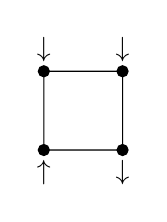
\begin{tikzpicture}
	\filldraw 	(0,0) circle(2pt) node[align=left, below]{$\uparrow$}-- 
				(0,1) circle(2pt) node[align=left, above]{$\downarrow$}-- 
				(1,1) circle(2pt) node[align=right, above]{$\downarrow$}-- 
				(1,0) circle(2pt) node[align=right, below]{$\downarrow$}-- (0,0);
	\end{tikzpicture}
	\caption{}
	\label{fig:4folddegen2by2lattice}
	\end{subfigure}
    \begin{subfigure}{0.45\linewidth}
    \centering
    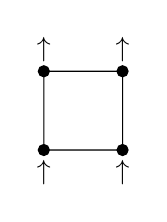
\begin{tikzpicture}
	\filldraw 	(0,0) circle(2pt) node[align=left, below]{$\uparrow$}-- 
				(0,1) circle(2pt) node[align=left, above]{$\uparrow$}-- 
				(1,1) circle(2pt) node[align=right, above]{$\uparrow$}-- 
				(1,0) circle(2pt) node[align=right, below]{$\uparrow$}-- (0,0);
	\end{tikzpicture}
	\caption{}
	\label{fig:2by2lattice}
    \end{subfigure}
    \caption{Simple 2x2 spin lattices with four - fold degeneracy (a), and single - fold degeneracy (b).}
\end{figure}
Consider Figure \ref{fig:4folddegen2by2lattice}, representing one of sixteen possible spin configurations in this system. This specific configuration has no net energy, which may be calculated through equation \eqref{specifichamiltonian}. Observe, however, that changing the position of the lonesome spin-up ($\uparrow$) to any of the other three corners of the lattice does not change the energy of the system - any configuration containing one spin up and three spin down is what we call a \textit{degenerate} configuration. In this case, the configuration is four - fold degenerate, which we choose to denote by $\mathcal{D}(s) = 4$. The magnetization of this particular configuration is $M = -2$, which may be calculated by equation \eqref{magnetization}. Such consideration need to be made for all sixteen possible spin configurations in the 2x2 spin lattice, and are summarized in the table below
\begin{table}[h!]
    \centering
    \caption{Tabular overview of associated degeneracies, energies and magnetizations for different spin - up configurations.}
    \begin{tabular}{c|c|c|c|c}
         \hline 
         Number of spin - up & $\mathcal{D}(s)$ & $E^{(s)}$ & $M^{(s)}$ & $|M|^{(s)}$ \\
         \hline
         4 & 1 & -$8J$ & 4 & 4\\
         3 & 4 & 0 & 2 & 2\\
         2 & 4 & 0 & 0 & 0\\
         2 & 2 & $8J$ & 0 & 0\\
         1 & 4 & 0 & -2 & 2\\
         0 & 1 & -$8J$ & -4 & 4\\
         \hline
    \end{tabular}
    
    \label{tab:latticevals}
\end{table}

Using the tabulated values in Table \ref{tab:latticevals}, and inserting them into equation \eqref{partitionfunc}, we arrive at
\begin{equation}
    Z_\beta = 2e^{8J\beta} + 2e^{-8J\beta} + 12 = 4\cosh(8J\beta) + 12
\end{equation}
Having established a closed form solution of $Z_\beta$, we may now unpack useful closed form solution of $\langle E \rangle$, $\langle |M| \rangle$, $C_V$ and $\mathcal{X}$ as functions of $\beta = 1/k_BT$. The expectation value of the energy as a function of $\beta$ becomes
\begin{equation}
    \langle E \rangle_\beta = -\frac{\partial}{\partial \beta}\ln Z_\beta = -8J\frac{\sinh(8J\beta)}{\cosh(8J\beta) + 3}
    \label{Energyclosedform}
\end{equation}
The heat capacity of the system at constant volume, $C_V$, correlates the energy variance at a temperature, to temperature it self through 
\[
C_V = \frac{1}{k_B T^2}\sigma^2_E = \frac{1}{k_B T^2}\left(\langle E^2 \rangle_\beta - \langle E \rangle^2_\beta\right)
\]
We may observe that the last term in the equation above is equivalent to
\begin{equation}
    C_V = \frac{1}{k_B T^2}\frac{\partial}{\partial \beta}\langle E \rangle _ \beta = \frac{192J^2}{k_B T^2}\frac{\cosh(8J\beta)}{\left(\cosh(8J\beta) + 3\right)^2}
    \label{heatcap}
\end{equation}
Moving on to the expected absolute magnetization, we may establish a closed form solution of this quantity by inserting values from Table \ref{tab:latticevals} into equation \eqref{magnetization}. This leads to
\begin{equation}
    \langle |M| \rangle_\beta = \frac{1}{Z_\beta}\left(8e^{8J\beta} + 16\right) = \frac{4\left(2e^{8J\beta} + 4\right)}{4\left(\cosh(8J\beta) + 3\right)} = \frac{2e^{8J\beta} + 4}{\cosh(8J\beta) + 3}
    \label{mabs}
\end{equation}
Observe simultaneously that 
\[
\langle M^2 \rangle_\beta = \frac{1}{Z_\beta}\left(32e^{8J\beta} + 32\right) = \frac{8e^{8J\beta} + 8}{\cosh(8J\beta) + 3}
\]
Together, these two expressions are related to the magnetic susceptibility $\mathcal{X}_\beta$ of the system through
\begin{equation}
    \mathcal{X}_\beta = \frac{1}{k_B T}\sigma^2_M = \frac{1}{k_B T}\left(\langle M^2 \rangle_\beta - \langle |M| \rangle^2_\beta \right) = \frac{1}{k_B T} \frac{\left(8e^{8J\beta}+8\right)\left(\cosh(8J\beta) + 3\right) - \left(2e^{8J\beta} + 4\right)^2}{\left(\cosh(8J\beta) + 3\right)^2}
    \label{suscept}
\end{equation}
At this point, we are able to determine analytical values for all of the physical quantities we may study in the 2x2 Ising model for a given temperature $T$. This allows us to study the performance of our algorithm closely, as we shall see in the Results section. 

\subsection{Critital Temperature, $T_C$}\label{sectioncritical}
In real materials, the number of particles (which would carry the spin-attribute) quickly becomes incredibly vast. A gram of solid material usually contains a number of particles within range of Avogadro's number ($\sim 10^{23}$), which puts the execution of the MHA not only at risk of overflow, but also gives computation times no ordinary student has the time, or willpower, to endure. The second-order phase transition we study in this project is characterized by a correlation length which spans the whole system. Since we are always limited, and severely so, to a finite lattice, we can devise so called finite size scaling relations, relating the behaviour of finite lattices with the results of infinitely large lattices. The critical temperature then scales as
\begin{align}
    T_C(\mathcal{L}) - T_C(\mathcal{L} = \infty) &= a\mathcal{L}^{-1/\nu}\label{critical}
\end{align}
The analytical value for the critical temperature was found by Lars Onsager \cite{statphys} to be approximately $2.269$ K.\\ \\
By setting $\nu = 1$, we can rewrite \eqref{critical} as
\begin{align}
    T_C(\mathcal{L}) &= a\mathcal{L}^{-1} + T_C(\mathcal{L}=\infty)\label{critical2}
\end{align}
This is a linear equation with the intercept as the critical temperature for an infinite lattice. We can then extract the critical temperature for several lattice sizes, and find the intercept by linear regression to approximate the analytical value.